% CMP4509 Introduction to Deep Learning -- Term project report template
% Compiles with pdfLaTeX + BibTeX (Overleaf: upload this folder or the .zip).
%
% The grey boxes are guides describing what is expected in each section.
% Keep them visible while writing. Before submitting, hide them all by
% changing \showguidesfalse to \showguidesfalse below.
\documentclass[11pt,a4paper]{article}

\usepackage[margin=2.5cm]{geometry}
\usepackage[T1]{fontenc}
\usepackage[utf8]{inputenc}
\usepackage{lmodern}
\usepackage{amsmath,amssymb,amsfonts}
\usepackage{graphicx}
\usepackage{booktabs}
\usepackage{multirow}
\usepackage{caption}
\usepackage{subcaption}
\usepackage{xcolor}
\usepackage{enumitem}
\usepackage[round]{natbib}
\usepackage[colorlinks=true,linkcolor=blue,citecolor=blue,urlcolor=blue]{hyperref}

% ---------------------------------------------------------------------------
% Guide boxes
\newif\ifshowguides
\showguidesfalse   % change to \showguidesfalse before submitting
\definecolor{guidebg}{gray}{0.93}
\definecolor{guideframe}{gray}{0.55}
\newcommand{\guide}[1]{%
  \ifshowguides
  \par\medskip\noindent
  \fcolorbox{guideframe}{guidebg}{%
    \begin{minipage}{\dimexpr\linewidth-2\fboxsep-2\fboxrule\relax}
      \small\textbf{Guide.}
      \begin{itemize}[leftmargin=1.2em,itemsep=1pt,topsep=2pt]
        #1
      \end{itemize}
    \end{minipage}}%
  \par\medskip
  \fi}
% ---------------------------------------------------------------------------

% Notation shortcuts (optional)
\newcommand{\R}{\mathbb{R}}
\newcommand{\E}{\mathbb{E}}
\newcommand{\vect}[1]{\mathbf{#1}}

\newcommand{\MNISTEnsembleAccuracy}{98.54 \pm 0.11}
\newcommand{\MNISTEnsembleError}{1.460 \pm 0.106}
\newcommand{\MNISTEnsembleNLL}{0.0558 \pm 0.0022}
\newcommand{\MNISTEnsembleBrier}{0.00247 \pm 0.00006}
\newcommand{\OODEnsembleID}{0.0788 \pm 0.0030}
\newcommand{\OODEnsembleOOD}{1.0222 \pm 0.0320}
\newcommand{\OODEnsembleGap}{0.9435 \pm 0.0309}
\newcommand{\OODEnsembleAUROC}{0.9653 \pm 0.0038}
\newcommand{\MNISTRandomAccuracy}{98.47 \pm 0.21}
\newcommand{\MNISTRandomError}{1.533 \pm 0.207}
\newcommand{\MNISTRandomNLL}{0.0567 \pm 0.0038}
\newcommand{\MNISTRandomBrier}{0.00250 \pm 0.00018}
\newcommand{\OODRandomID}{0.0770 \pm 0.0097}
\newcommand{\OODRandomOOD}{0.8056 \pm 0.0404}
\newcommand{\OODRandomGap}{0.7286 \pm 0.0363}
\newcommand{\OODRandomAUROC}{0.9346 \pm 0.0118}
\newcommand{\MNISTATAccuracy}{98.61 \pm 0.09}
\newcommand{\MNISTATError}{1.390 \pm 0.089}
\newcommand{\MNISTATNLL}{0.0498 \pm 0.0039}
\newcommand{\MNISTATBrier}{0.00225 \pm 0.00015}
\newcommand{\OODATID}{0.0766 \pm 0.0073}
\newcommand{\OODATOOD}{1.0193 \pm 0.0209}
\newcommand{\OODATGap}{0.9426 \pm 0.0153}
\newcommand{\OODATAUROC}{0.9668 \pm 0.0023}
\newcommand{\MNISTDropoutAccuracy}{97.32 \pm 0.22}
\newcommand{\MNISTDropoutError}{2.680 \pm 0.217}
\newcommand{\MNISTDropoutNLL}{0.0986 \pm 0.0070}
\newcommand{\MNISTDropoutBrier}{0.00420 \pm 0.00037}
\newcommand{\OODDropoutID}{0.1161 \pm 0.0053}
\newcommand{\OODDropoutOOD}{0.5354 \pm 0.1175}
\newcommand{\OODDropoutGap}{0.4192 \pm 0.1189}
\newcommand{\OODDropoutAUROC}{0.7779 \pm 0.0736}
\newcommand{\ToyMSEIDRMSE}{5.421 \pm 0.360}
\newcommand{\ToyMSEIDNLL}{7785.0 \pm 10950.3}
\newcommand{\ToyMSEIDCoverage}{13.58 \pm 5.52}
\newcommand{\ToyMSELeftRMSE}{83.133 \pm 2.895}
\newcommand{\ToyMSELeftNLL}{355.1 \pm 155.8}
\newcommand{\ToyMSELeftCoverage}{0.00 \pm 0.00}
\newcommand{\ToyMSERightRMSE}{33.767 \pm 1.035}
\newcommand{\ToyMSERightNLL}{522.0 \pm 719.3}
\newcommand{\ToyMSERightCoverage}{7.54 \pm 9.85}
\newcommand{\ToyGaussianIDRMSE}{5.024 \pm 0.073}
\newcommand{\ToyGaussianIDNLL}{15967.0 \pm 4320.1}
\newcommand{\ToyGaussianIDCoverage}{46.57 \pm 0.45}
\newcommand{\ToyGaussianLeftRMSE}{79.187 \pm 0.305}
\newcommand{\ToyGaussianLeftNLL}{7526602.8 \pm 70051.8}
\newcommand{\ToyGaussianLeftCoverage}{0.00 \pm 0.00}
\newcommand{\ToyGaussianRightRMSE}{39.170 \pm 10.714}
\newcommand{\ToyGaussianRightNLL}{6.0 \pm 2.5}
\newcommand{\ToyGaussianRightCoverage}{69.65 \pm 39.55}
\newcommand{\ToyGaussianATIDRMSE}{5.019 \pm 0.081}
\newcommand{\ToyGaussianATIDNLL}{171.7 \pm 94.2}
\newcommand{\ToyGaussianATIDCoverage}{61.60 \pm 0.88}
\newcommand{\ToyGaussianATLeftRMSE}{80.530 \pm 0.472}
\newcommand{\ToyGaussianATLeftNLL}{4030276.6 \pm 1599794.2}
\newcommand{\ToyGaussianATLeftCoverage}{0.00 \pm 0.00}
\newcommand{\ToyGaussianATRightRMSE}{35.442 \pm 1.039}
\newcommand{\ToyGaussianATRightNLL}{5.0 \pm 0.2}
\newcommand{\ToyGaussianATRightCoverage}{67.86 \pm 4.42}
\newcommand{\ToyDeepIDRMSE}{5.063 \pm 0.109}
\newcommand{\ToyDeepIDNLL}{131.1 \pm 121.7}
\newcommand{\ToyDeepIDCoverage}{50.07 \pm 2.03}
\newcommand{\ToyDeepLeftRMSE}{79.728 \pm 0.454}
\newcommand{\ToyDeepLeftNLL}{3961.5 \pm 3417.6}
\newcommand{\ToyDeepLeftCoverage}{0.00 \pm 0.00}
\newcommand{\ToyDeepRightRMSE}{33.814 \pm 3.390}
\newcommand{\ToyDeepRightNLL}{4.7 \pm 0.3}
\newcommand{\ToyDeepRightCoverage}{89.33 \pm 17.91}

\title{Reproducing ``\textit{Simple and Scalable Predictive Uncertainty Estimation using Deep Ensembles}''\\[0.3em]
\large CMP4509 Introduction to Deep Learning --- Term Project Report}
\author{Student 1 [Full Name, ID] \and Student 2 [Full Name, ID] \and Student 3 [Full Name, ID]}
\date{26 November 2026}
\begin{document}
\maketitle
\begin{abstract}
Neural networks can be accurate while assigning excessive confidence to unfamiliar inputs. We reproduce selected experiments of \citet{lakshminarayanan2017simple}: cubic toy regression, MNIST classification and MNIST/NotMNIST out-of-distribution (OOD) uncertainty. Three training seeds and a resource-scaled PyTorch implementation run on both a local GPU and an actual free Google Colab Tesla T4. We consistently use Colab as the primary reporting environment and local runs as supplementary evidence. At five members, adversarially trained ensembles achieve $\MNISTATAccuracy\%$ MNIST accuracy and $\OODATAUROC$ entropy-based OOD AUROC, versus $\MNISTDropoutAccuracy\%$ and $\OODDropoutAUROC$ for five MC Dropout passes. These results support the selected classification/OOD trend, with no significance claim. Toy regression is only a partial reproduction: all methods have zero left-OOD 95\% noisy-observation coverage in every seed in both environments. We preserve these failures, distinguish learned and between-model variance, document all deviations and verify the identity of the reused OOD checkpoints.
\end{abstract}

\section{Introduction}
\label{sec:intro}
Predictive uncertainty asks how much trust to place in a prediction, including when the input differs from the training distribution. Accuracy alone does not describe the reliability of predicted probabilities. A digit classifier, for example, must still return a digit distribution for an unfamiliar letter. Low entropy in that situation can conceal model misspecification.

\citet{lakshminarayanan2017simple} propose independently trained probabilistic networks, proper scoring rules and optional adversarial training as a practical alternative to approximate Bayesian uncertainty estimation. We test three specific claims: whether learned variance and ensembling reproduce Figure~1's sensible regression uncertainty, whether ensembles improve classification scores relative to sampled dropout in Figure~2(a), and whether their uncertainty increases more strongly on unknown classes in Figure~3(a). We do not reproduce the paper's regression benchmark suite, SVHN, ImageNet or every reported number. A failure of the selected toy uncertainty claim is a central result rather than a result to discard.

\section{Background and Method}
\label{sec:method}
\subsection{Predictive distributions and proper scoring rules}
Let $\mathcal D=\{(x_n,y_n)\}_{n=1}^N$, with $x_n\in\R^d$. A network with parameters $\theta$ specifies a predictive distribution $p_\theta(y\mid x)$. A minibatch input has shape $[B,d]$. For regression the network outputs mean and variance tensors $[B,1]$; for classification it outputs probabilities $[B,K]$.

A loss is proper if the true conditional distribution $q$ minimizes its conditional expectation. For log loss,
\begin{align}
\E_q[-\log p(Y\mid x)]
&=-\E_q\log q(Y\mid x)+\E_q\log\frac{q(Y\mid x)}{p(Y\mid x)}\\
&=H(q)+D_{\rm KL}(q\Vert p)\geq H(q).\label{eq:proper}
\end{align}
The first term does not depend on the reported $p$; nonnegative KL divergence makes $p=q$ optimal. This explains why negative log-likelihood (NLL) rewards a distribution rather than only a point estimate \citep{gneiting2007proper}. Propriety is a population property and does not guarantee finite-data calibration or good extrapolation.

\subsection{Gaussian NLL and a positive variance}
Assume $Y\mid x\sim\mathcal N(\mu_\theta(x),v_\theta(x))$, $v=\sigma^2>0$. Taking minus the logarithm of the density gives
\begin{equation}
-\log\left[(2\pi v)^{-1/2}e^{-(y-\mu)^2/(2v)}\right]
=\tfrac12\log(2\pi)+\tfrac12\log v+\frac{(y-\mu)^2}{2v}.\label{eq:gaussian}
\end{equation}
The residual term discourages a small variance around errors, while $\log v$ penalizes arbitrarily broad predictions. Our output $a(x)\in\R$ becomes $v(x)=\log(1+e^{a(x)})+10^{-6}$ via numerically stable softplus. Fixed $v$ makes NLL proportional to MSE, but MSE alone does not learn input-dependent variance. An empirical variance of MSE-network predictions has no explicit observation-noise model.

Our Gaussian toy targets use $\widetilde y=(y-\bar y)/s_y$, with statistics from training data only. Returning to physical units requires $\mu=\bar y+s_y\widetilde\mu$ and $v=s_y^2\widetilde v$. Density transformation adds $\log s_y$ to normalized NLL. Training omits constants independent of parameters; reported NLL includes the density constant and original-unit scaling.

\subsection{Mixture prediction and total variance}
For $M$ independently trained networks, define $p_E(y\mid x)=M^{-1}\sum_m p_{\theta_m}(y\mid x)$. For Gaussian members, introduce the uniformly sampled member index $Z$. Conditional expectation gives
\begin{align}
\mu_E&=\E_Z\E[Y\mid Z]=M^{-1}\sum_m\mu_m,\\
\E[Y^2]&=M^{-1}\sum_m(v_m+\mu_m^2),\\
v_E&=\E[Y^2]-\mu_E^2
=\underbrace{M^{-1}\sum_m v_m}_{\text{within-member component}}
+\underbrace{M^{-1}\sum_m(\mu_m-\mu_E)^2}_{\text{between-member component}}.\label{eq:mixture}
\end{align}
This is the law of total variance, $\E_Z\operatorname{Var}(Y\mid Z)+\operatorname{Var}_Z\E(Y\mid Z)$. The components are commonly interpreted as aleatoric-like observation ambiguity and epistemic-like model disagreement. They are model-dependent estimates, not guaranteed identification of true noise and posterior uncertainty. Members can share a systematic extrapolation error.

The variance in Eq.~\eqref{eq:mixture} uses divisor $M$, because it is the variance of a uniform mixture, not an unbiased sample variance estimate. We use its moment-matched Gaussian for plotted bands and moment NLL. The exact mixture density $M^{-1}\sum_m\mathcal N(y;\mu_m,v_m)$ can have very different NLL; both are retained in the repository. A $\mu_E\pm z\sqrt{v_E}$ prediction interval is conditional on this Gaussian approximation, not a confidence interval for a seed-averaged score.

\subsection{Adversarial training, random perturbations and dropout}
For a small input perturbation $\delta$, Taylor expansion gives $\ell(x+\delta,y)\simeq\ell(x,y)+\delta^Tg$, where $g=\nabla_x\ell$. Maximizing each coordinate under $|\delta_i|\leq\epsilon_i$ yields
\begin{equation}
\delta_i^*=\epsilon_i\operatorname{sign}(g_i),\qquad
x'=x+\delta^*,\qquad L_{\rm AT}=\ell(\theta,x,y)+\ell(\theta,x',y).\label{eq:fgsm}
\end{equation}
FGSM therefore targets a locally high-loss direction \citep{goodfellow2015explaining}; random signs of the same size need not increase loss. We set $\epsilon_i$ to 1\% of the training-data range of coordinate $i$, clipping image perturbations to $[0,1]$. The clean-plus-perturbed objective is a sum, not a half-weighted average. The paper motivates this local smoothing but does not establish universal OOD robustness.

Initialization and shuffled data order provide diversity while each ensemble member sees the full designated training split. Bagging is unnecessary here and would reduce distinct training examples per member. MC Dropout instead samples masks of one trained model at evaluation \citep{gal2016dropout}. Our three dropout layers stay active at $p=0.1$, while the parent model and every BatchNorm layer stay in evaluation mode. Otherwise updated BatchNorm statistics would confound the uncertainty calculation.

\subsection{Classification probabilities, scores and entropy}
For logits $z\in\R^K$, $p_k=e^{z_k}/\sum_j e^{z_j}$ and cross-entropy $-\sum_k\mathbf1[y=k]\log p_k=-\log p_y$ equals categorical NLL. The ensemble probability tensor has shape $[M,N,K]$ and is averaged on its first axis: $\bar p_{nk}=M^{-1}\sum_m p_{mnk}$. Softmax is nonlinear, so averaging logits is a different estimator. We compute
\begin{align}
\mathrm{NLL}&=-N^{-1}\sum_n\log\bar p_{n,y_n},\\
\mathrm{BS}&=(NK)^{-1}\sum_{n,k}(\bar p_{nk}-\mathbf1[y_n=k])^2.\label{eq:classmetrics}
\end{align}
Metrics use float64 accumulation; classification NLL floors target probabilities at $10^{-12}$ for numerical stability. The paper's $1/K$ Brier normalization matters for numerical comparison. Under true categorical probabilities $q$, its conditional expectation is
$K^{-1}(\|p-q\|_2^2+1-\|q\|_2^2)$, minimized at $p=q$; this also establishes propriety.

Predictive entropy, measured in nats, is
\begin{equation}
H_n=-\sum_k\bar p_{nk}\log\bar p_{nk},\qquad 0\log0:=0,\qquad
0\leq H_n\leq\log K.\label{eq:entropy}
\end{equation}
For the uniform $u_k=1/K$, $D_{\rm KL}(p\Vert u)=\log K-H(p)\geq0$ proves the upper bound; each $-p_k\log p_k\geq0$ proves the lower bound. Thus $K=10$ gives $[0,\log10]$. Entropy of the mixture is not mean member entropy: two certain members predicting different classes each have zero entropy, but their equal mixture has $H=\log2$. In general, concavity gives $H(\bar p)\geq M^{-1}\sum_m H(p_m)$; their difference measures disagreement. Predictive entropy includes ambiguity and disagreement rather than isolating epistemic uncertainty.

For our added OOD analysis, set MNIST label 0, NotMNIST label 1 and score $s=H$. Then
\begin{equation}
\mathrm{AUROC}=\Pr(s_{\rm OOD}>s_{\rm ID})+\tfrac12\Pr(s_{\rm OOD}=s_{\rm ID}),\quad
\Delta_H=\overline H_{\rm OOD}-\overline H_{\rm ID}.\label{eq:ood}
\end{equation}
These summarize ranking and mean separation, respectively, and require no chosen detection threshold. They supplement the paper's entropy histograms. Neither guarantees reliable detection for every input.

\section{Experimental Setup}
\label{sec:setup}
\subsection{Fixed protocol and compute}
We use run seeds $42,123,2026$ throughout. One ensemble is one experimental run, irrespective of its five members. For a score $a_s$ over $S=3$ seeds,
\begin{equation}
\bar a=S^{-1}\sum_s a_s,\qquad s_a=\sqrt{\frac{\sum_s(a_s-\bar a)^2}{S-1}}.
\end{equation}
Error bars and tables use this sample SD (ddof=1), not a standard error or confidence interval. All seeds share the fixed data/split, so this spread does not measure variation across datasets.

All primary results use the completed Colab Tesla T4 runs. Local RTX~4070~Ti~SUPER results are supplementary. Colab uses Python~3.13.16, PyTorch~2.14.1+cu130, CUDA~13.0 and NumPy~2.4.6. The local stack uses PyTorch~2.11.0+cu128 and CUDA~12.8. Floating-point and optimization trajectories need not match bitwise across these environments. Final-delivery preparation involved no retraining, inference rerun or hyperparameter tuning.

\subsection{Toy regression}
We preserve one 20-point CSV generated with data seed 42, $x\sim U[-4,4]$, $y=x^3+\eta$, $\eta\sim\mathcal N(0,9)$. MSE uses a $1$--$50$--$1$ ReLU MLP (151 parameters); Gaussian networks use $1$--$50$--$2$ (202 parameters). Every model uses 3,000 full-batch Adam epochs \citep{kingma2015adam}, lr $0.01$ for MSE and $0.001$ for Gaussian NLL, default betas $(0.9,0.999)$, optimizer epsilon $10^{-8}$ and zero weight decay. The Gaussian models normalize targets using training mean $12.5197773$ and population SD $20.4321270$. FGSM epsilon is $0.06608958$, 1\% of the observed input range. Seed experiments use member seed $100s+j$, $j=0,\ldots,4$; single models use $j=0$.

We compare five-member MSE ensembles, single Gaussian NLL, single Gaussian NLL+AT and five-member Gaussian NLL ensembles without AT. The latter decomposes variance using Eq.~\eqref{eq:mixture}. The evaluation grid has 400 points on $[-6,6]$ and 20 fresh noisy responses at each point, with fixed evaluation seed 20261122. ID is $[-4,4]$ (266 grid points); each OOD side has 67 points. No evaluation targets enter training. Main curves show $\pm3$ SD as in the paper; separately added 95\% coverage uses $\pm1.95996398454$ SD on noisy targets. MSE proxy variance has evaluation floor $10^{-6}$ in original $y^2$ units. The small own data draw, target normalization, chosen rates and full-batch budget are documented deviations; exact original toy optimization trajectories are not available.

\subsection{MNIST classification}
The MLP is $784$--$200$--$200$--$200$--$10$, with three ReLU and BatchNorm layers, totaling 240,610 trainable parameters. MC Dropout adds $p=0.1$ after each ReLU. Raw uint8 inputs become float32 $[0,1]$ vectors of length 784 without additional normalization. A train-only permutation with split seed 4509 allocates 55,000 images to training and 5,000 to validation; the official 10,000-image test set remains separate. This holdout and the 10-epoch budget are deviations from an exact standard-training-set reproduction.

The saved final profile uses Adam lr $0.1$, betas $(0.9,0.999)$, epsilon $10^{-8}$, no weight decay, batch size 100 and evaluation batch size 1,000. Default PyTorch Linear initialization and BatchNorm initialization are seeded. Training shuffles each epoch; epsilon uses training-only per-pixel ranges (69 constant pixels have zero epsilon). Ensemble, Ensemble+R and Ensemble+AT each train five models per seed; MC Dropout trains one and uses up to five stochastic passes. Thus $3(5+5+5+1)=48$ models support $M=1,2,3,4,5$. Test metrics use the final epoch, not test-selected checkpoints. Earlier tuning history is not completely evidenced in the final archives; we therefore do not invent a validation-search procedure or claim a new optimization study.

\subsection{OOD evaluation and evidence}
The MNIST test set has 10,000 images. NotMNIST small/test contains 18,726 PNGs, of which two known unreadable images are excluded, leaving all 18,724 valid 28-by-28 grayscale images. We preserve float32/255 scaling, native light-foreground polarity and no added normalization, resizing, augmentation or subsampling. The pinned archive SHA-256 is provided in repository metadata. For each method and seed, $M=1,3,5$ are prefixes of the same five-member/pass probability stack, yielding 36 seed rows and 12 summaries.

The 48 OOD checkpoint hashes agree with the completed MNIST Colab audit and the associated Figure~2(a) CSV. No OOD model is trained. Sequential loaders include final partial batches. The dropout RNG stream is seeded once per dataset/method stream; BatchNorm buffers remain fixed. Windows' case-insensitive and Linux's case-sensitive path ordering initially produced a false tensor-hash mismatch. The Colab adapter permutes images, labels and IDs together to the saved reference order: 16,719 of 18,724 positions change, no pixels change, and tensor/order hashes then agree. The actual completed Colab alignment JSON records this correction. Checkpoint source, data, configuration and runtime signatures protect cache reuse; source errors never trigger local-model fallback or training.

Recorded times have different scopes: Toy's complete notebook workload is 333.21~s, MNIST invocation is 1,228.19~s, OOD's 24 inference groups total 15.91~s, and its complete inference invocation is 52.42~s. The OOD group times include loading and small audit probes, but exclude preparation/plotting; these are not normalized runtime benchmarks.

\section{Results}
\label{sec:results}
\subsection{Figure 1: an important partial failure}
Figure~\ref{fig:toy} displays the first predeclared seed (42), not a visually selected best run. Table~\ref{tab:toy} aggregates all three seeds. The main plot uses $\pm3$ SD; the separately calculated coverage is for $\pm1.96$ SD on fresh noisy observations.

\begin{figure}[htbp]
\centering
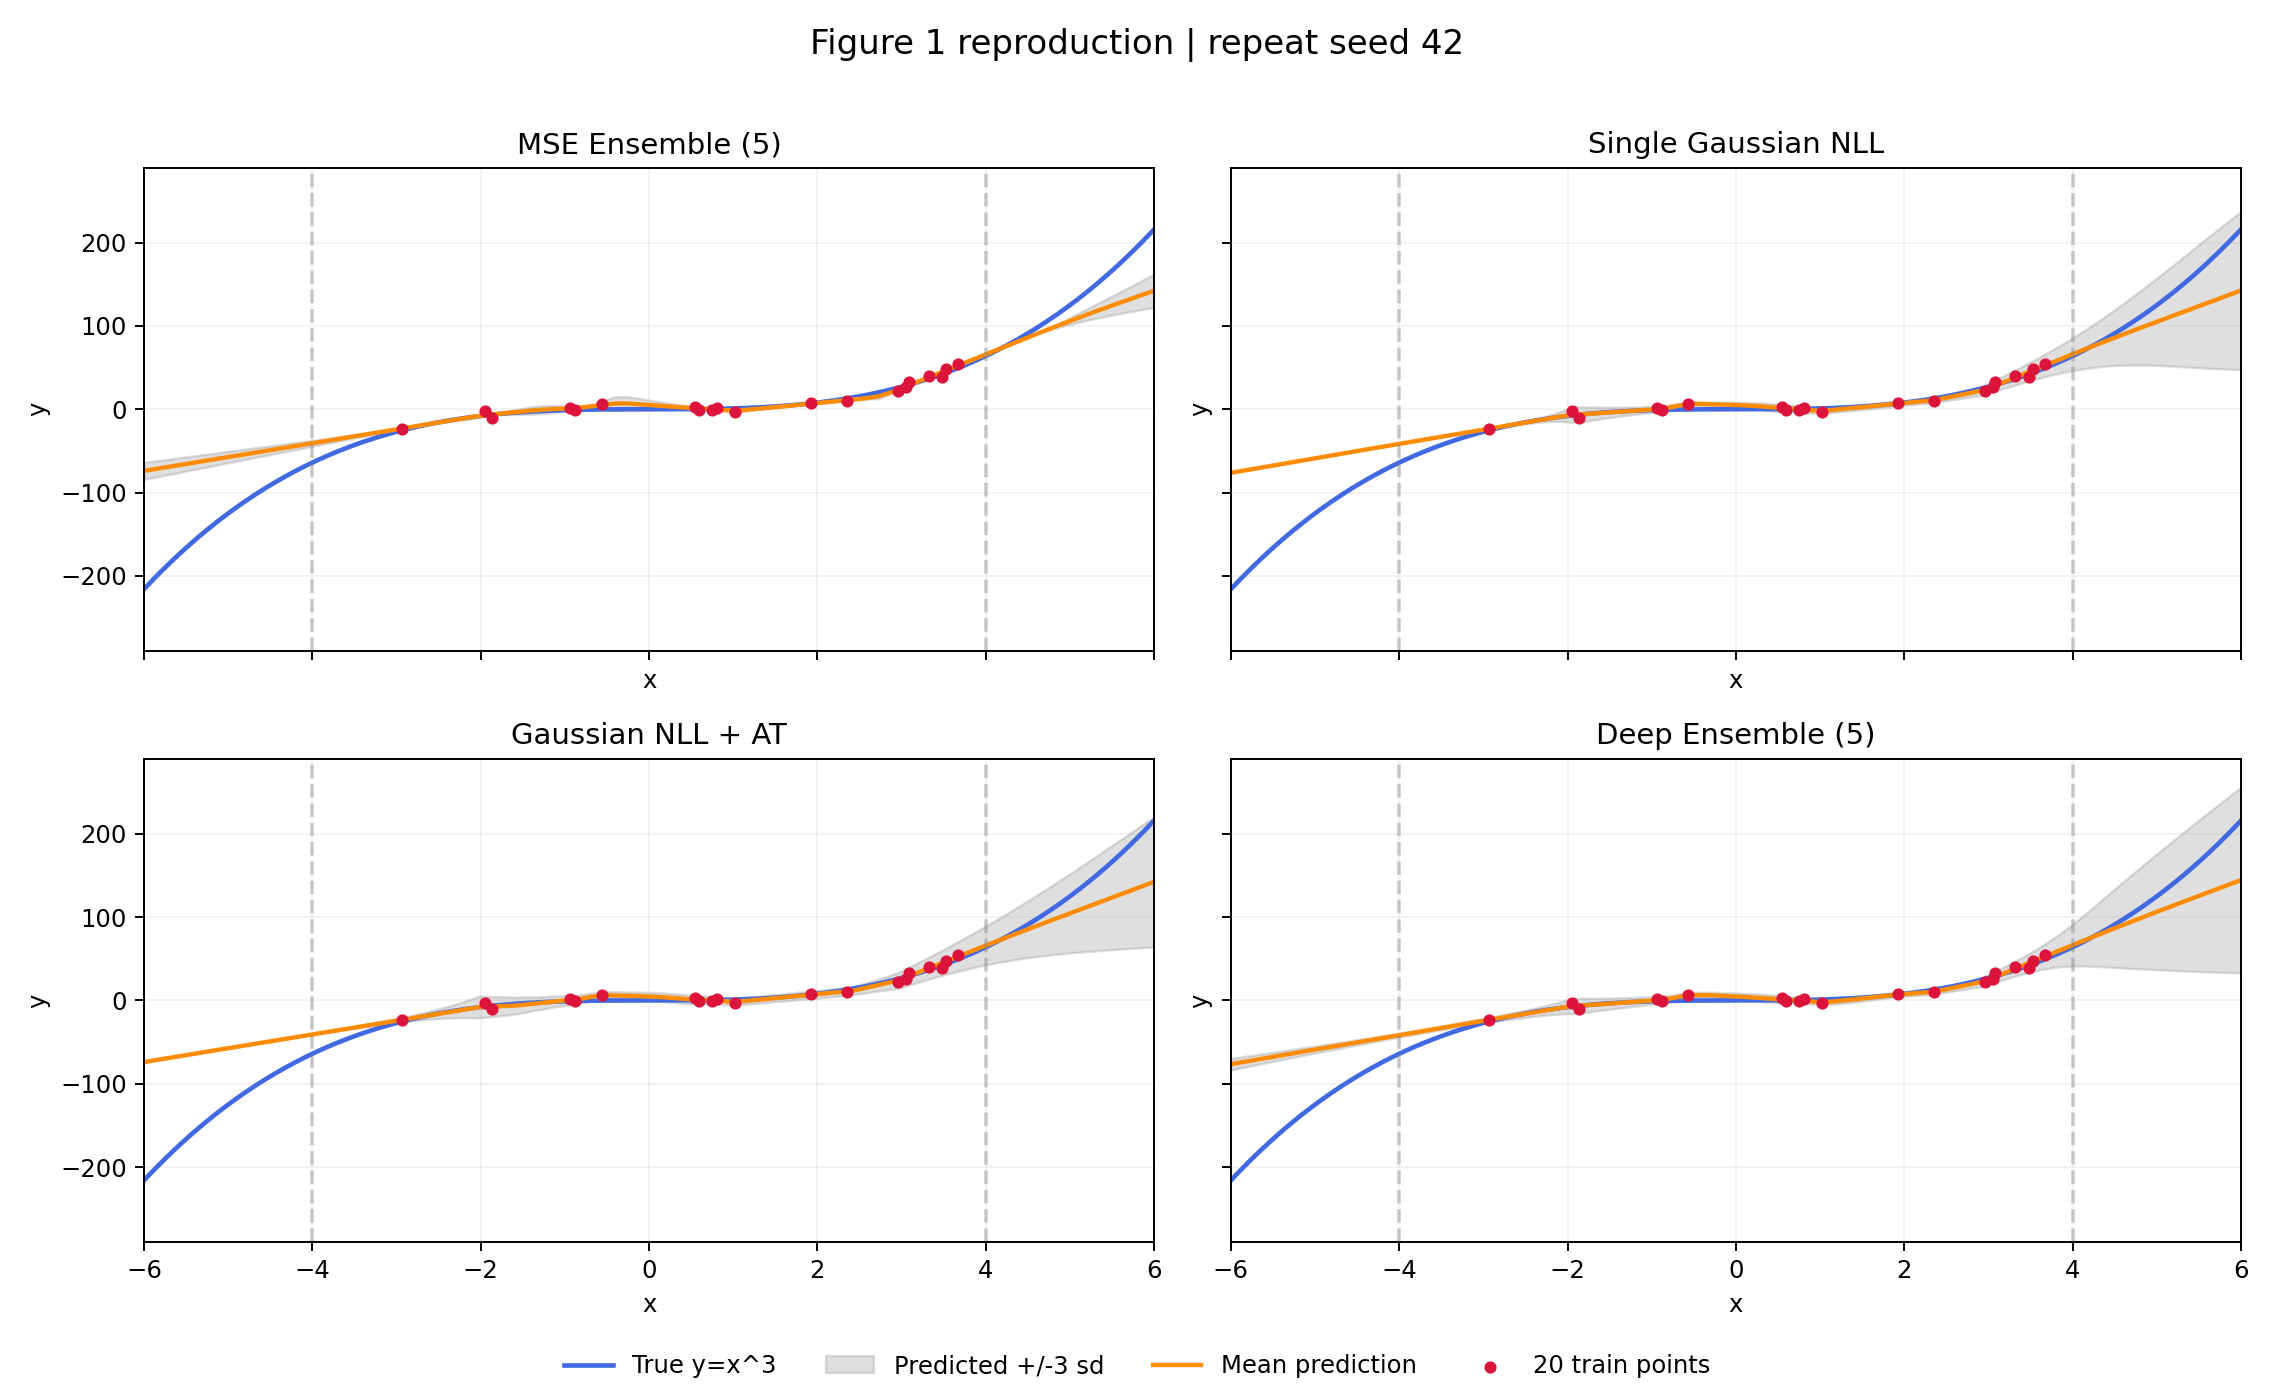
\includegraphics[width=\linewidth]{figures/figure1_toy_colab.png}
\caption{Actual Colab toy reproduction, seed 42. Four original prediction panels compare empirical MSE variance, learned single Gaussian variance, single-model AT and a Gaussian NLL ensemble. Red points are the same 20 training observations; blue is $x^3$; gray bands are predicted mean $\pm3$ SD. All seed panels are retained in the repository. This illustrates the selected Figure~1 comparison, but the data draw/optimization differ from the original paper and the left extrapolation is poor.}
\label{fig:toy}
\end{figure}


\begin{table}[htbp]
\centering\small
\caption{Toy Colab results, mean $\pm$ sample SD over three training seeds. ID clean-curve RMSE and moment-Gaussian NLL on noisy targets are distinct metrics. Coverage uses a separate 95\% prediction interval and noisy targets. The paper's Figure~1 is qualitative and supplies no directly comparable numeric regional targets.}
\label{tab:toy}
\begin{tabular}{lrrr}
\toprule Method & ID RMSE & ID NLL & Left OOD coverage (\%)\\\midrule
MSE Ensemble & $\ToyMSEIDRMSE$ & $\ToyMSEIDNLL$ & $\ToyMSELeftCoverage$\\
Single Gaussian & $\ToyGaussianIDRMSE$ & $\ToyGaussianIDNLL$ & $\ToyGaussianLeftCoverage$\\
Gaussian + AT & $\ToyGaussianATIDRMSE$ & $\ToyGaussianATIDNLL$ & $\ToyGaussianATLeftCoverage$\\
Deep Ensemble & $\ToyDeepIDRMSE$ & $\ToyDeepIDNLL$ & $\ToyDeepLeftCoverage$\\
\bottomrule
\end{tabular}
\end{table}

Deep Ensemble left-OOD RMSE is $\ToyDeepLeftRMSE$, compared with $\ToyDeepIDRMSE$ in ID. Its ID/right-OOD noisy 95\% coverages are $\ToyDeepIDCoverage\%$ and $\ToyDeepRightCoverage\%$, respectively. Every method/seed has zero left coverage in both environments. Exact-mixture Deep Ensemble NLL is 5,469.82 $\pm$ 5,062.57 in ID and approximately $4.98\times10^6$ on the left; the reported moment-matched NLL is a different density approximation. Full regional RMSE/NLL/coverage/width/component tables, including these large failures, are retained.

\subsection{Figure 2(a): probabilistic classification quality}
Figure~\ref{fig:mnist} shows all tested sizes; Table~\ref{tab:mnist} gives $M=5$. Error, NLL and paper-normalized Brier scores favor ensembles over the sampled dropout baseline in this protocol. For reference, the original Figure~2(a) plots a larger ensemble-size range and reports qualitative ordering; it does not supply an exact matching CSV for our ten-epoch/holdout setup.

\begin{figure}[htbp]
\centering
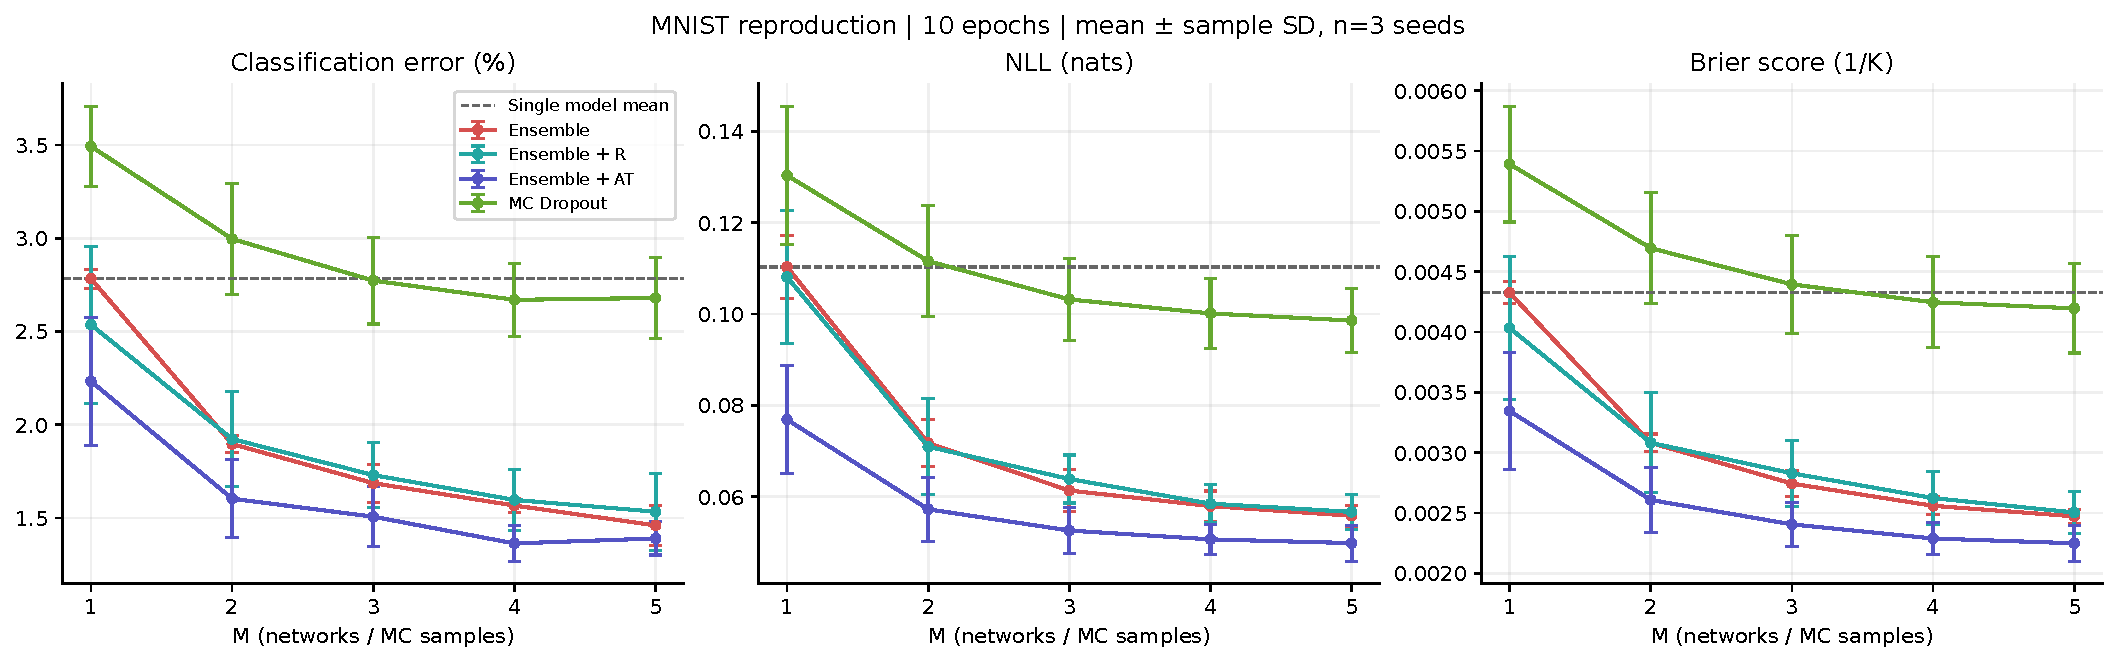
\includegraphics[width=\linewidth]{figures/figure2a_mnist_colab.pdf}
\caption{Actual Colab Figure~2(a) reproduction: MNIST classification error, NLL and $1/K$-normalized Brier score versus $M=1,2,3,4,5$. Each point aggregates run seeds 42,123,2026; error bars are sample SD, not confidence intervals. MC Dropout uses $M$ stochastic passes of one model per seed.}
\label{fig:mnist}
\end{figure}


\begin{table}[htbp]
\centering\small
\caption{MNIST Colab, $M=5$, mean $\pm$ sample SD over three seeds. Error is a percentage; NLL is in nats; Brier includes $1/K$. Training budget, split and ensemble-size range differ from the original Figure~2(a).}
\label{tab:mnist}
\begin{tabular}{lrrr}\toprule Method & Error (\%) & NLL & Brier\\\midrule
Ensemble & $\MNISTEnsembleError$ & $\MNISTEnsembleNLL$ & $\MNISTEnsembleBrier$\\
Ensemble + R & $\MNISTRandomError$ & $\MNISTRandomNLL$ & $\MNISTRandomBrier$\\
Ensemble + AT & $\MNISTATError$ & $\MNISTATNLL$ & $\MNISTATBrier$\\
MC Dropout & $\MNISTDropoutError$ & $\MNISTDropoutNLL$ & $\MNISTDropoutBrier$\\\bottomrule
\end{tabular}
\end{table}

The accuracies are $\MNISTEnsembleAccuracy\%$, $\MNISTRandomAccuracy\%$, $\MNISTATAccuracy\%$ and $\MNISTDropoutAccuracy\%$. Improvement is not universally monotonic: AT mean error rises from 1.363\% at $M=4$ to 1.390\% at $M=5$, and dropout from 2.670\% to 2.680\%. We report these small reversals without a significance claim.

\subsection{Figure 3(a): unseen classes and residual overconfidence}
Figure~\ref{fig:ood} and Table~\ref{tab:ood} use exactly the Figure~2(a) Colab checkpoints. The histogram trend supports higher unseen-class uncertainty with larger ensembles in this setting. NotMNIST mean entropy rises from $M=1$ to 5 more for each ensemble variant than for dropout. Low-entropy mass on some letters remains, so the result does not establish uniformly safe OOD behavior.

\begin{figure}[htbp]
\centering
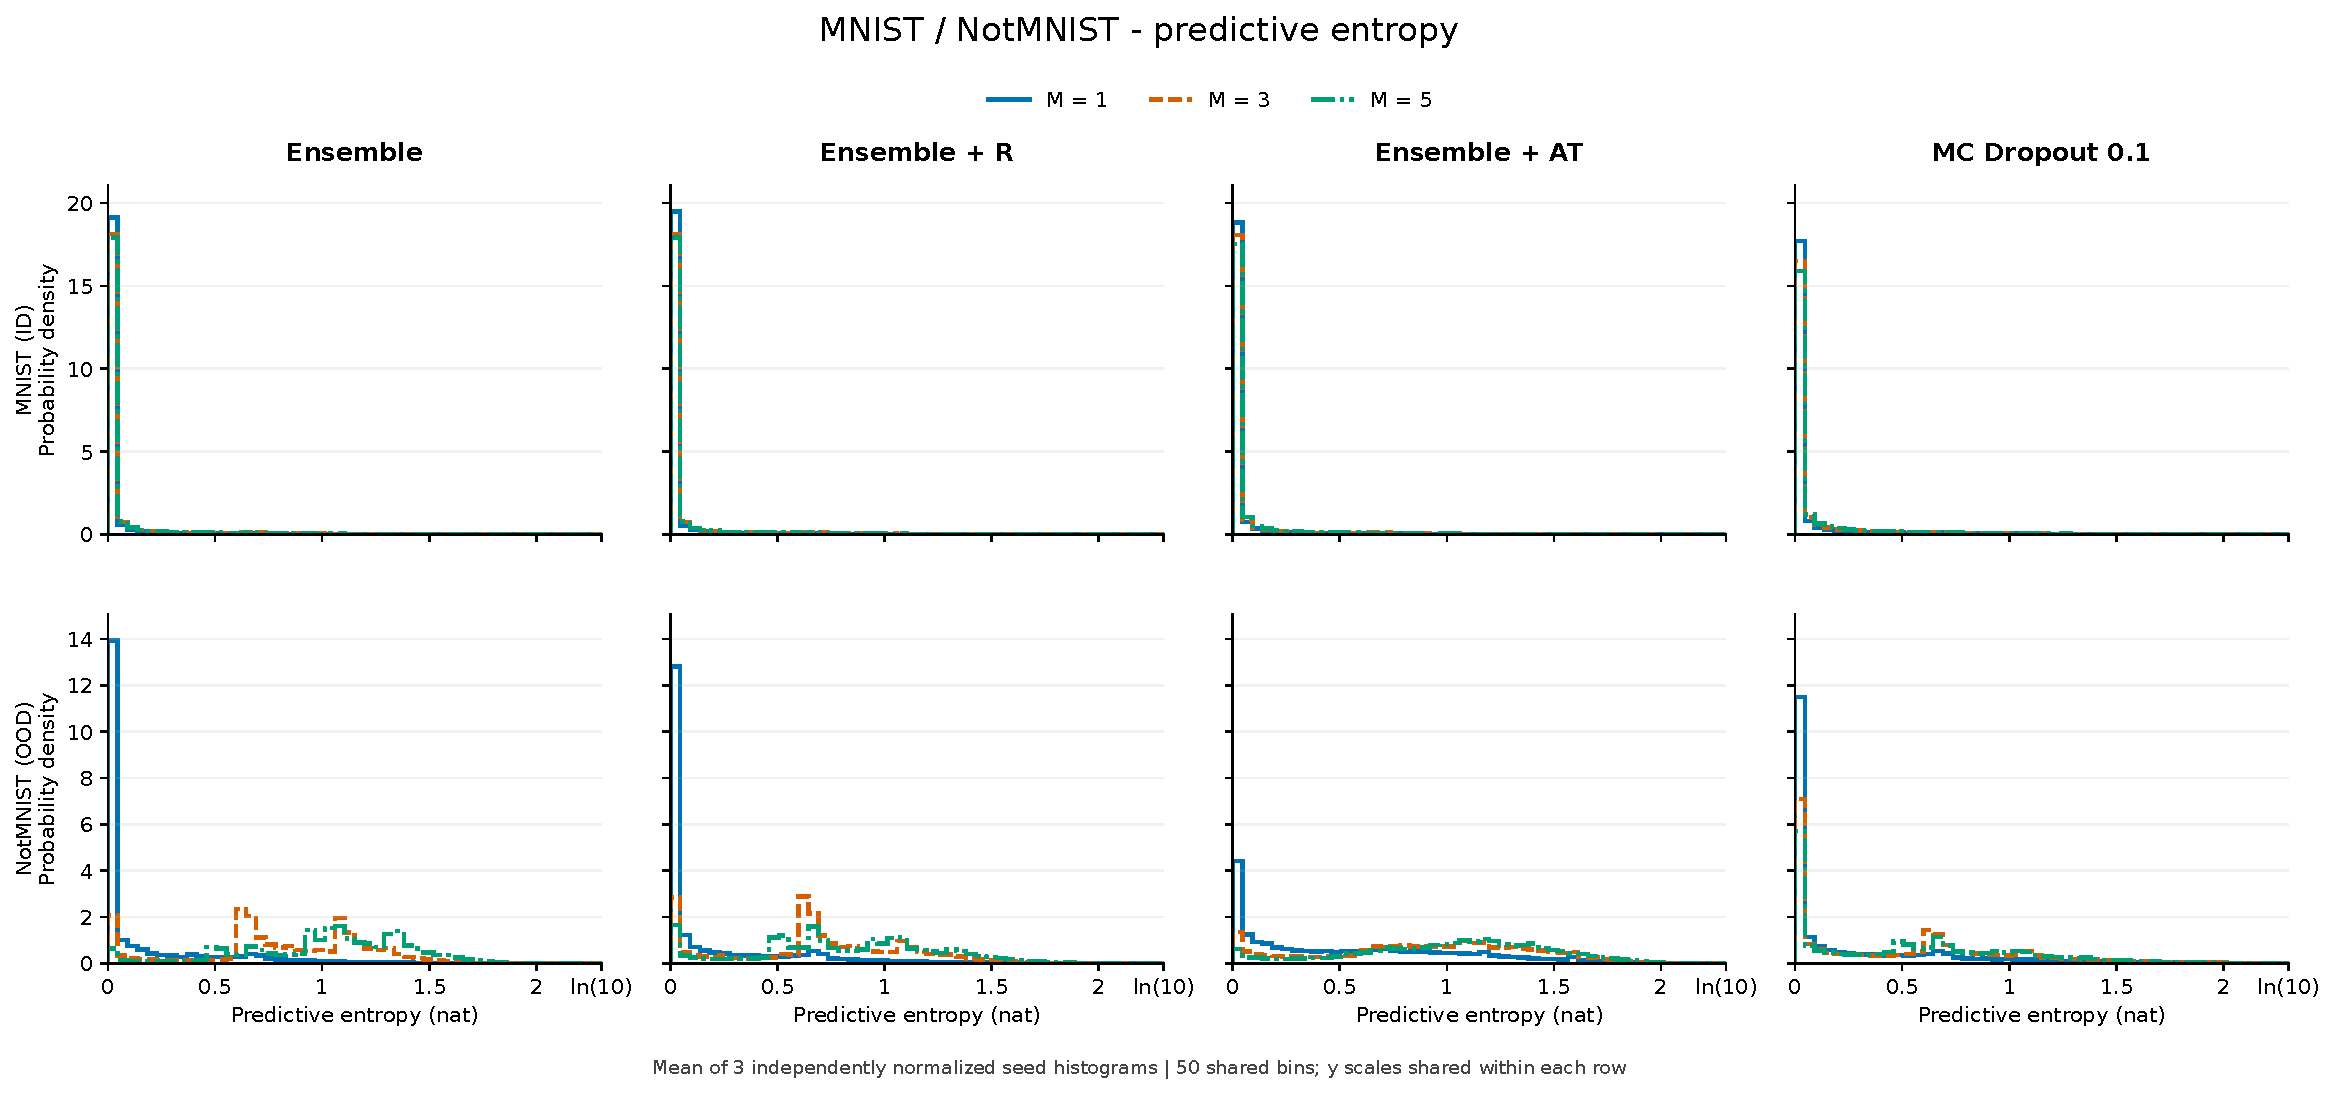
\includegraphics[width=\linewidth]{figures/figure3a_ood_colab.pdf}
\caption{Actual Colab Figure~3(a) reproduction. Top row: 10,000 MNIST digits (ID); bottom row: 18,724 valid NotMNIST letters (OOD). Columns: Ensemble, +R, +AT, MC Dropout. Curves use $M=1,3,5$, whereas the original shows $M=1,5,10$. Histograms share 50 bins on $[0,\log10]$, normalize each seed to unit area, then average the three densities. Scales are shared within each row.}
\label{fig:ood}
\end{figure}


\begin{table}[htbp]
\centering\small
\caption{Added OOD analyses at $M=5$ (not original Figure~3(a) numeric metrics). Mean $\pm$ sample SD, $n=3$. Gap is mean OOD minus mean ID entropy in nats. AUROC treats MNIST as 0, NotMNIST as 1 and higher entropy as more OOD-like.}
\label{tab:ood}
\begin{tabular}{lrrr}\toprule Method & Mean OOD entropy & Entropy gap & AUROC\\\midrule
Ensemble & $\OODEnsembleOOD$ & $\OODEnsembleGap$ & $\OODEnsembleAUROC$\\
Ensemble + R & $\OODRandomOOD$ & $\OODRandomGap$ & $\OODRandomAUROC$\\
Ensemble + AT & $\OODATOOD$ & $\OODATGap$ & $\OODATAUROC$\\
MC Dropout & $\OODDropoutOOD$ & $\OODDropoutGap$ & $\OODDropoutAUROC$\\\bottomrule
\end{tabular}
\end{table}

Local supplementary $M=5$ AUROCs are 0.9544 $\pm$ 0.0106, 0.9433 $\pm$ 0.0219, 0.9653 $\pm$ 0.0060 and 0.7860 $\pm$ 0.1115 in the same method order. The negative local Ensemble $M=1$, seed 123 AUROC of 0.3790 is retained. OOD digit accuracy is not defined for letter labels outside the ten digit classes. All 36 MNIST accuracy/NLL/Brier consistency comparisons in the actual Colab OOD evidence match their own classifier run within the original tolerances.

\section{Discussion}
\label{sec:discussion}
The selected classification and unknown-class results support the paper's qualitative ensemble-versus-dropout direction under our resource-scaled protocol. AT has the lowest mean MNIST NLL/Brier at $M=5$, and often improves OOD separation. Random directions are not equivalent to FGSM: they use the same perturbation scale but do not maximize local loss. Nevertheless, the modest AT-versus-plain-ensemble OOD AUROC difference must be interpreted alongside seed spread; neither statistical significance nor universal method superiority is established. MSE proxy variance and learned Gaussian variance are distinct uncertainty constructions, and the toy experiment shows that even the latter plus model diversity can fail.

Toy reproduction is partial. The left-side error is large while the learned within-member variance often approaches its floor, and between-member disagreement does not cover shared extrapolation error. Similar ReLU extrapolation and maximum-likelihood variance collapse in data-sparse regions are plausible explanations. These remain hypotheses: no controlled causal ablation was performed. The persistence of zero left coverage locally and on T4 makes the failure robust to this environment comparison, but does not prove its mechanism.

Our scope excludes the original larger ensemble grids, other architectures/datasets and broader calibration studies. Three training seeds and a fixed toy data draw give limited statistical evidence; sample SD is not a significance test. NLL/Brier and OOD rankings cannot alone establish full calibration. Ensemble training/storage scales with the number of networks, whereas MC Dropout shares one network's parameters but still requires multiple forward passes. Saved invocation times use unequal scopes and do not constitute a compute-efficiency benchmark. Software and GPU differences are plausible contributors to local/Colab discrepancies; we did not isolate them experimentally. All complete tables, seed figures, source/config/checkpoint hashes, executed notebooks, test logs and deviations are supplied rather than selecting a favorable environment for each method.

\section{Conclusion}
\label{sec:conclusion}
We reproduced three selected Deep Ensembles experiments with three seeds and verified actual T4 evidence. Classification and MNIST/NotMNIST uncertainty show the expected qualitative ensemble advantage under the tested budget. Toy regression provides a substantive counterexample to uniformly reliable extrapolation: left-OOD coverage fails in every run. The appropriate conclusion is a limited, transparent reproduction with documented successes and failures, not an exact or complete replication of the paper.

\section*{Contributions}
Student 1 [Full Name, ID]: [Replace with verified implementation, derivation, experiment or writing contributions and evidence from files or commits].

Student 2 [Full Name, ID]: [Replace with verified contributions and evidence from files or commits].

Student 3 [Full Name, ID]: [Replace with verified contributions and evidence from files or commits]. All members must independently understand the complete method, code and derivations. These placeholders do not assert a division of work.

\section*{Use of AI Tools}
ChatGPT and Codex assisted code implementation/debugging, notebook and test preparation, saved-results auditing, documentation, mathematical exposition and report/presentation drafting and checking. Numerical results originate in saved program outputs from actual experiments, not generated values. The students must independently verify and understand all derivations and implementation decisions, complete the genuine contribution record, and approve this assisted draft before submission. No other AI tools are claimed.

\section*{Code}
\url{https://github.com/aligk97/deep-ensembles-reproduction}

The existing repository is public. The accompanying clean final-delivery tree contains runnable notebook sources, local/Colab result tables, evidence and this report. Publication of that final tree still requires the students' reviewed push/merge; this preparation did not publish changes. Notebook order is Toy Regression, MNIST Classification, then OOD using the classifier's Drive RUN\_ID or complete export ZIP. Saved preparation checks are distinguished from the recorded real T4 experiments.

\bibliographystyle{plainnat}
\bibliography{references}
\end{document}
